%%%%%%%%%%%%%%%%%%%%%%%%%%%%%%%%%%%%%%%%%
% Beamer Presentation
% LaTeX Template
% Version 2.0 (27/IX/15)
%
% This template has been downloaded from http://www.LaTeXTemplates.com
% and modified by Semen Martynov <semen.martynov@gmail.com>
%
% License:
% CC BY-NC-SA 3.0 (http://creativecommons.org/licenses/by-nc-sa/3.0/)
%
%%%%%%%%%%%%%%%%%%%%%%%%%%%%%%%%%%%%%%%%%

%----------------------------------------------------------------------------------------
%	PACKAGES AND THEMES
%----------------------------------------------------------------------------------------

\documentclass{beamer}

\mode<presentation> {

% The Beamer class comes with a number of default slide themes
% which change the colors and layouts of slides. Below this is a list
% of all the themes, uncomment each in turn to see what they look like.

%\usetheme{default}
%\usetheme{AnnArbor}
%\usetheme{Antibes}
%\usetheme{Bergen}
%\usetheme{Berkeley}
%\usetheme{Berlin}
%\usetheme{Boadilla}
%\usetheme{CambridgeUS}
%\usetheme{Copenhagen}
%\usetheme{Darmstadt}
%\usetheme{Dresden}
%\usetheme{Frankfurt}
%\usetheme{Goettingen}
%\usetheme{Hannover}
%\usetheme{Ilmenau}
%\usetheme{JuanLesPins}
%\usetheme{Luebeck}
\usetheme{Madrid}
%\usetheme{Malmoe}
%\usetheme{Marburg}
%\usetheme{Montpellier}
%\usetheme{PaloAlto}
%\usetheme{Pittsburgh}
%\usetheme{Rochester}
%\usetheme{Singapore}
%\usetheme{Szeged}
%\usetheme{Warsaw}

% As well as themes, the Beamer class has a number of color themes
% for any slide theme. Uncomment each of these in turn to see how it
% changes the colors of your current slide theme.

%\usecolortheme{albatross}
%\usecolortheme{beaver}
%\usecolortheme{beetle}
%\usecolortheme{crane}
%\usecolortheme{dolphin}
%\usecolortheme{dove}
%\usecolortheme{fly}
%\usecolortheme{lily}
%\usecolortheme{orchid}
%\usecolortheme{rose}
%\usecolortheme{seagull}
%\usecolortheme{seahorse}
%\usecolortheme{whale}
%\usecolortheme{wolverine}

%\setbeamertemplate{footline} % To remove the footer line in all slides uncomment this line
%\setbeamertemplate{footline}[page number] % To replace the footer line in all slides with a simple slide count uncomment this line

%\setbeamertemplate{navigation symbols}{} % To remove the navigation symbols from the bottom of all slides uncomment this line
\setbeamertemplate{caption}[numbered] % Image numbers
}

%%%% Charset (don't forget about texlive-lang-cyrillic)
\usepackage{cmap}							% make PDF files searchable and copyable
\usepackage[utf8x]{inputenc}				% accept different input encodings
\usepackage[T2A]{fontenc}					% russian font
\usepackage[russian]{babel}					% multilingual support (T2A)

%%%% Graphics
%\usepackage[dvipsnames]{xcolor}			% driver-independent color extensions
\usepackage{graphicx}						% enhanced support for graphics
\usepackage{wrapfig}						% produces figures which text can flow around

%%%% Math
\usepackage{amsmath}						% American Mathematical Society (AMS) math facilities
\usepackage{amsfonts}						% fonts from the AMS
\usepackage{amssymb}						% additional math symbols

%%%% Typograpy (don't forget about cm-super)
\usepackage{microtype}						% subliminal refinements towards typographical perfection
%\linespread{1.3}							% line spacing
\setlength{\parindent}{0pt}					% we don't want any paragraph indentation
\usepackage{parskip}						% some distance between paragraphs

%%%% Tables
\usepackage{booktabs}						% Allows the use of \toprule, \midrule and \bottomrule in tables
%\usepackage{tabularx}						% tables with variable width columns
%\usepackage{multirow}						% for tabularx
%\usepackage{hhline}							% for tabularx

%%%% Graph
%\usepackage{tikz}							% package for creating graphics programmatically
%\usetikzlibrary{arrows}						% edges for tikz

%%%% Other
%\usepackage{url}							% verbatim with URL-sensitive line breaks
%\usepackage{fancyvrb}						% sophisticated verbatim text (with box)

\makeatletter
\def\verbatim{\tiny\@verbatim \frenchspacing\@vobeyspaces \@xverbatim}
\makeatother

%----------------------------------------------------------------------------------------
%	TITLE PAGE
%----------------------------------------------------------------------------------------

\title[Кэш-память]{Исследование работы Кэш-памяти\\ центрального процессора} % The short title appears at the bottom of every slide, the full title is only on the title page

\author{Чёрная команда} % Your name
\institute[СПбПУ] % Your institution as it will appear on the bottom of every slide, may be shorthand to save space
{
Санкт-Петербургский политехнический университет Петра Великого \\ % Your institution for the title page
\medskip
\textit{Антон Абрамов <abramov91@mail.ru>\\
Владислав Бусаров <happyfanik@yandex.ru>\\
Сергей Дедков <dsv.mail@yandex.ru>\\
Семён Мартынов <semen.martynov@gmail.com>\\
Николай Патраков <noon.vlg@gmail.com>} % Your email address
}
\date{\today} % Date, can be changed to a custom date

\begin{document}

\begin{frame}
\titlepage % Print the title page as the first slide
\end{frame}

\begin{frame}
\frametitle{Содержание} % Table of contents slide, comment this block out to remove it
\tableofcontents % Throughout your presentation, if you choose to use \section{} and \subsection{} commands, these will automatically be printed on this slide as an overview of your presentation
\end{frame}

%----------------------------------------------------------------------------------------
%	PRESENTATION SLIDES
%----------------------------------------------------------------------------------------

%------------------------------------------------
\section{Назначение кэш памяти}
%------------------------------------------------

\begin{frame}
\frametitle{Понятие кэш-памяти}

\begin{block}{Кэш (от фр. cacher -- "прятать")}
промежуточный буфер с быстрым доступом, содержащий информацию, которая может быть запрошена с наибольшей вероятностью. Доступ к данным в кэше осуществляется быстрее, чем выборка исходных данных из более медленной памяти или удаленного источника, однако её объём существенно ограничен по сравнению с хранилищем исходных данных.
\end{block}

Понятие предложено в 1967 году Лайлом Джонсоном (редактором журнала "IBM Systems Journal") как замена термину "высокоскоростной буфер" при описании памяти в разрабатываемой модели 85 из серии IBM System/360.

\end{frame}

%------------------------------------------------

\begin{frame}
\frametitle{Нужна ли кэш-память в современных системах?}

Оперативная память представляет собой динамическую память с произвольным доступом (Dynamic Random Access Memory, DRAM), а кэш процессора выполняется на базе статической оперативной памяти (Static Random Access Memory, SRAM).\\~\\

Рассмотрим память DDR3-1600 9-9-9-27 (tCL-tRCD-tRP-tRAS): эффективная частота составляет 1600 МГц, это скорость с которой данные поступают на внешнюю шину в пакетном режиме доступа, а реальная частота ядра памяти составляет всего 200 МГц.\\~\\

С момента активации нужной строки памяти и до появления данных на шине пройдет промежуток времени, равный tCL+tRCD, то есть 18 тактов. С учетом того что частота работы ядра памяти DDR3-1600 составляет 200 МГц, это время равно 90 нс. Если частота работы процессора составляет 3 ГГц, то это означает, что процессор должен будет дожидаться нужных данных (простаивать) минимум 270 тактов!

\end{frame}

%------------------------------------------------

\begin{frame}
\frametitle{Почему DRAM-память не заменить SRAM-памятью?}

Каждая ячейка DRAM-памяти состоит из одного полевого транзистора и одного конденсатора, ячейка SRAM-памяти -- как минимум из шести полевых транзисторов (есть варианты с числом транзисторов 8 и 12). Об этом рассказывал проф. Мелехин.\\~\\

В результате:
\begin{itemize}
\item Модули SRAM-памяти были бы меньшего объема в сравнении с модулями DRAM-памяти
\item Их цена (даже при равном объёме) была бы выше
\item Существенно возросла бы проблема кэширования периферийных устройств
\item Пришлось бы перерабатывать систему кэширования, которая на данный момент работает достаточно хорошо =)
\end{itemize}

\end{frame}

%------------------------------------------------
\section{Принцип работы кэша процессора}
%------------------------------------------------

\begin{frame}
\frametitle{Принцип работы кэша процессора}

\begin{figure}
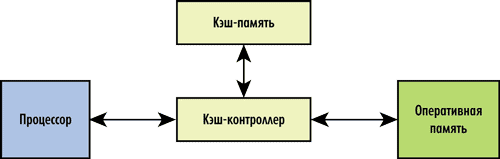
\includegraphics[scale=0.65]{Pic_1}
\caption{Структура кэш-памяти процессора}
\end{figure}

Кэш-контроллер перехватывает запросы к оперативной памяти и определяет, имеется ли копия затребованных данных в кэше. Если есть (cache hit), то данные извлекаются из кэша, если нет (cache miss) -- тогда запрос переадресуется к оперативной памяти.

\end{frame}

%------------------------------------------------

\begin{frame}
\frametitle{Стратегии кэширования}

Кэш-контроллер должен уметь предсказывать какие данные потребуются процессору в будущем и загружать их в кэш (упреждающая загрузка данных)\\~\\

\begin{itemize}
\item On demand -- обращение к оперативной памяти происходит только в случае кэш-промаха
\item Look Ahead -- алгоритмы упреждающей спекулятивной загрузки данных в кэш основанные на предположении, что данные из оперативной памяти обрабатываются последовательно, в порядке возрастания адресов
\begin{itemize}
\item Look Through -- загрузка данных из памяти может либо начинаться после фиксации кэш-промаха
\item Look Aside -- загрузка осуществляться параллельно с проверкой наличия соответствующей копии данных и до кэш-попадания (очень эффективна, но увеличивается энергопотребление процессора)
\end{itemize}
\end{itemize}

\end{frame}

%------------------------------------------------

\begin{frame}
\frametitle{Политики замещения данных в кэш-памяти}

Кэш всегда полон; новые данные можно занести только путем замещения каких-­либо старых.
\begin{itemize}
\item[Rnd] (Random) замещаемые данные выбираются случайным образом
\item[LFU] (Least Frequently Used) -- в первую очередь замещаются данные, у которых самая низкая частота обращений (требует наличия счетчика удачных запросов в каждой строке кэша)
\item[LRU] (Least Recently Used) -- замещаются те данные, к которым дольше всего не обращались
\item[LRR] (Least Recently Replaced) -- замещаются те данные, которые были загружены раньше всех

\end{itemize}

\end{frame}


%------------------------------------------------
\section{Организация кэша}
%------------------------------------------------

\begin{frame}
\frametitle{Организация кэша}

Из чего формируется кэш-строка (cache-line):
\begin{itemize}
\item Счетчик возраста строк, для реализации политики замещения на основе алгоритма LRU
\item 32-разрядный (четырехбайтный) адрес памяти, используемый контроллером для проверки промахов/попаданий. Адрес сохраняемого слова принято называть тегом (tag)
\item Блок данных фиксированного размера (степени двойки -- 2, 4, 8, 16 и т.д.), идущих подряд в оперативной памяти. Он называется размером кэш строки.

\end{itemize}

\end{frame}

%------------------------------------------------

\begin{frame}
\frametitle{Организация кэша}

\begin{figure}
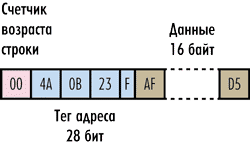
\includegraphics[scale=0.7]{Pic_2}
\caption{Пример кэш-строки размером 16 байт}
\end{figure}

Размер кэш строки всегда равен степени двойки, а данные не пересекаются. Тогда размер тега (в битах) равен $32 - log_{2} S$, где S -- размер кэш строки в байтах.

Если размер кэш строки равен 16 байт -- то размер тега адреса 28 бита. Для строки из 32 байт -- 27 бит адреса, 64 бай адресуются 26 битами.
\end{frame}

%------------------------------------------------

\begin{frame}
\frametitle{Организация кэша}

Объём кэша можно рассматривать как полный, и как полезный.

Пусть имеется кэш размером 32 Кбайт и длина строки составляет 128 байт.  Такой кэш будет содержать 256 строк (32 Кбайт/128 байт). Каждая строка имеет тег размером 25 бит (32 – $log_2$ 128). Кроме того, добавим счетчик старения, содержащий 8 бит ($log_2$ 256). То есть к каждой строке добавляется еще 33 служебных бита. А всего таких служебных бит будет 8'448 или 1'056 байт. Соответственно полный объем кэша составит чуть более 33 Кбайт.

В рассмотренном нами кэше мы не учитывали так называемые биты модификации, которые также добавляются в каждой строке кэша и необходимы для поддержания когерентности.

\end{frame}


%------------------------------------------------
\section{Понятие ассоциативности кэша}
%------------------------------------------------

\begin{frame}
\frametitle{Полностью ассоциативная кэш-память (Fully associative)}

\begin{figure}
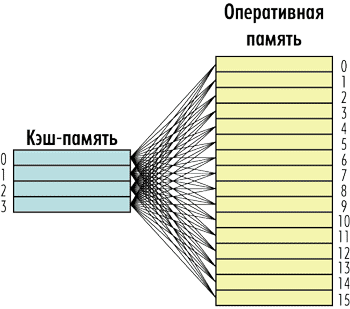
\includegraphics[scale=0.53]{Pic_3}
\caption{Структура полностью ассоциативной кэш-памяти}
\end{figure}

Чтобы определить, имеются ли запрошенные процессором данные в кэш-памяти, нужно перебрать все кэш строки.

\end{frame}

%------------------------------------------------

\begin{frame}
\frametitle{Кэш-память с прямым отображением (Direct mapping)}

\begin{figure}
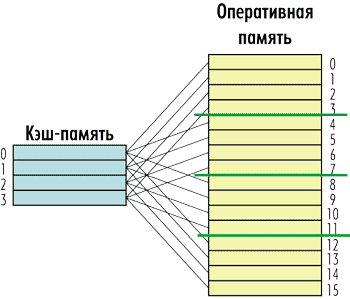
\includegraphics[scale=0.55]{Pic_4}
\caption{Структура кэш-памяти с прямым отображением}
\end{figure}

Каждой строке кэш-памяти соответствует несколько (строго определенных) строк оперативной памяти.

\end{frame}

%------------------------------------------------

\begin{frame}
\frametitle{Кэш-память с прямым отображением (Direct mapping)}

Соотношение между номерами строк оперативной памяти и номерами кэш-­строк:

\begin{center}
$N_{cache} = (N_{memory})mod(N_{max\_cache})$
\end{center}

Где:
\begin{itemize}
\item $N_{cache}$ номер кэш строки
\item $N_{memory}$ номер строки оперативной памяти
\item $N_{max\_cache}$ количество строк кэш-памяти
\item $mod$ функция получения остатка от деления
\end{itemize}

\end{frame}

%------------------------------------------------

\begin{frame}
\frametitle{Кэш-память с прямым отображением (Direct mapping)}

Перейдём от строк оперативной памяти к адресному пространству.

\begin{center}
$N_{memory} = (ADDR)div(CACHE\_LINE\_SIZE)$
\end{center}

Где:
\begin{itemize}
\item $ADDR$ адрес элемента в оперативной памяти
\item $CACHE\_LINE\_SIZE$ размер кэш-строки
\item $div$ функция целочисленного деления
\end{itemize}

Количество строк кэш-памяти можно выразить следующим образом:

\begin{center}
$N_{max\_cache} = (CACHE\_SIZE)div(CACHE\_LINE\_SIZE)$
\end{center}
\end{frame}

%------------------------------------------------

\begin{frame}
\frametitle{Кэш-память с прямым отображением (Direct mapping)}

Тогда выражение, определяющее номер строки кэш-памяти, в которую попадет элемент оперативной памяти с адресом $ADDR$, запишется в виде:

\begin{align*}
N_{cache} =& [(ADDR)div(CACHE\_LINE\_SIZE)] \\
& mod [(CACHE\_SIZE)div(CACHE\_LINE\_SIZE)]
\end{align*}

\end{frame}

%------------------------------------------------

\begin{frame}
\frametitle{Наборно-ассоциативный кэш (N-way cache)}

\begin{figure}
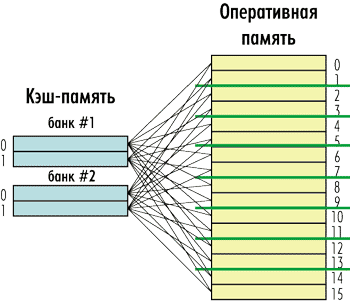
\includegraphics[scale=0.5]{Pic_5}
\caption{Структура наборно-ассоциативного кэша}
\end{figure}

Кэш состоит из нескольких независимых банков (сегментов), каждый из которых представляет собой кэш с прямым отображением, а сами банки полностью ассоциативны по отношению к оперативной памяти.

\end{frame}

%------------------------------------------------

\begin{frame}
\frametitle{Наборно-ассоциативный кэш (N-way cache)}

Количество банков кэша называется его степенью ассоциативности или канальностью (way). То есть может быть 2-канальный (2-way), 4-канальный (4-way), 8-канальный (8-way) и т.д.\\~\\

Поскольку каждый банк кэш-памяти является сегментом памяти с прямым отображением, в нем действует то же правило, что и для кэш-памяти с прямым отображением, то есть:

\begin{center}
$N_{bank\_cache} = (N_{memory})mod(N_{max\_bank\_cache})$
\end{center}

Где:
\begin{itemize}
\item $N_{bank\_cache}$ номер кэш строки в банке памяти
\item $N_{max\_bank\_cache}$ количество строк кэш-памяти в банке
\item $N_{memory}$ номер строки оперативной памяти
\end{itemize}

\end{frame}

%------------------------------------------------

\begin{frame}
\frametitle{Наборно-ассоциативный кэш (N-way cache)}

Количество строк кэш-памяти в банке определяется соотношением:

\begin{center}
$N_{max\_bank\_cache} = \frac{N_{max\_cache}}{N}$
\end{center}

Где:
\begin{itemize}
\item $N_{max\_cache}$ количество строк в кэш-памяти
\item $N$ степень ассоциативности (количество банков или каналов).
\end{itemize}

\end{frame}

%------------------------------------------------
\section{Эксперимент}
%------------------------------------------------

\begin{frame}
\frametitle{Постановка задачи}
Исследовать характеристики обращение к памяти для программ из бенчмарка Ливерморские циклы, ядра 1-9.

Используя результаты исследования, определить оптимальную для этой вычислительной нагрузки конфигурацию кэш-памяти \textbf{общим объемом} 0,5 Мбайт;

Параметры:
\begin{itemize}
\item m -- число строк
\item n -- число слов в строке
\item k -- коэффициент ассоциативности
\end{itemize}
\end{frame}

%------------------------------------------------

\begin{frame}
\frametitle{Ливерморские циклы}
"Ливерморские циклы" появился в середине 60-х годов и состоит из фрагментов программ, имеющих реальное хождение в Ливерморской Национальной лаборатории им. Лоуренса в США.\\~\\

Считается, что Ливерморские циклы -- это типичный набор программ для решения численных задач. В этих фрагментах используются различные вычислительные алгоритмы: сеточные, последовательные, волновые, что существенно с точки зрения соответствия вычислительных и аппаратных структур.
\end{frame}

%------------------------------------------------

\begin{frame}
\frametitle{Ливерморские циклы}
\begin{enumerate}
\item Hydro fragment
\item ICCG excerpt (Incomplete Cholesky Conjugate Gradient)
\item Inner product
\item Banded linear equations
\item Tri-diagonal elimination, below diagonal
\item General linear recurrence equations
\item Equation of state fragment
\item ADI integration
\item Integrate predictors
\end{enumerate}
Исходный код \url{https://github.com/SemenMartynov/SPbPU_ComputingSystems/tree/master/lab2/livermorec.txt}
\end{frame}

%------------------------------------------------

\begin{frame}
\frametitle{Порядок решения}

Для решения задачи было принято решение использовать средство динамического анализа Intel Pin:\\~\\

\begin{enumerate}
\item На 32-битной системе мы запустили pintool (для оптимизированной и не оптимизированной версии ливерморских циклов), генерирующий журнал обращений к памяти
\item На С++ реализовали модель работы кэш-памяти 32-битного процессора (использовалась стратегии кэширования On demand, и алгоритм LFU для замещения)
\item По итогам моделирования получили таблицу с количеством кэш промахов и попаданий при различных коэффициентах ассоциативности, количестве и длине кэш строк.
\end{enumerate}

\end{frame}

%------------------------------------------------

\begin{frame}[fragile] % Need to use the fragile option when verbatim is used in the slide
\frametitle{Сборка с использованием gcc 4.6.3.}

\begin{block}{Компиляция с максимальной оптимизацией}
\begin{verbatim}
$ gcc livermorec.c -o livermorec-mxopt -O3
$ /opt/pin/pin -t /opt/pin/source/tools/SimpleExamples/obj-ia32/pinatrace.so -- ./livermorec-mxopt
$ mv pinatrace.out livermorec-mxopt.out
\end{verbatim}
\end{block}
Реальное время работы программы с оснасткой 0m13.114s

\begin{block}{Компиляция без оптимизации}
\begin{verbatim}
$ gcc livermorec.c -o livermorec-noopt -O0
$ /opt/pin/pin -t /opt/pin/source/tools/SimpleExamples/obj-ia32/pinatrace.so -- ./livermorec-noopt
$ mv pinatrace.out livermorec-no/opt.out
\end{verbatim}
\end{block}
Реальное время работы программы с оснасткой 0m13.442s

\begin{block}{результаты компиляции (журналы отличаются)}
\begin{verbatim}
$ du -hsBk livermorec*
20K          livermorec.c
8K           livermorec-mxopt
1756K        livermorec-mxopt.out
12K          livermorec-noopt
1764K        livermorec-noopt.out
\end{verbatim}
\end{block}

\end{frame}

%------------------------------------------------

\begin{frame}
\frametitle{Особенности модели кэша}

При разработке модели кэша мы заложили следующие особенности:\\~\\

\begin{enumerate}
\item Проверка на размер. Общий объём кэша вычисляется в зависимости от переданных параметров и не может превышать 512 Кбайт
\item Если запрошенный из памяти кусок данных требует обращения к нескольким кэш-строкам, то кэш-попадание засчитывается только в случае если все куски были кэшированы и обращение к памяти не потребовалось
\item Модель ориентирована на вычисление промахов и попаданий, а не на эффективное хранение адресов (тегов)
\end{enumerate}

\end{frame}


%------------------------------------------------

\begin{frame}[fragile] % Need to use the fragile option when verbatim is used in the slide
\frametitle{Результат для оптимизированной версии}

\begin{block}{Лучшие результаты}
\begin{verbatim}

/---------------------------------------------------\
| C.Lines |  Words  |  Assoc. | Miss ctr |  Hit ctr |
|---------|---------|---------|----------|----------|
|       4 |       1 |       2 |     7000 |    39250 |
|       8 |       1 |       4 |     7000 |    39250 |
|      16 |       1 |       8 |     7000 |    39250 |
|       8 |       1 |       2 |     9459 |    36791 |
|      16 |       1 |       4 |     9459 |    36791 |
|      32 |       1 |       8 |     9459 |    36791 |
\---------------------------------------------------/

\end{verbatim}
\end{block}

\begin{block}{Худшие результаты}
\begin{verbatim}

                                                    /---------------------------------------------------\
                                                    | C.Lines |  Words  |  Assoc. | Miss ctr |  Hit ctr |
                                                    |---------|---------|---------|----------|----------|
                                                    |     512 |       8 |       2 |    41840 |     4410 |
                                                    |    1024 |       8 |       4 |    41840 |     4410 |
                                                    |    2048 |       8 |       8 |    41840 |     4410 |
                                                    |    1024 |       8 |       2 |    44195 |     2055 |
                                                    |    2048 |       8 |       4 |    44195 |     2055 |
                                                    |    4096 |       8 |       8 |    44195 |     2055 |
                                                    \---------------------------------------------------/

\end{verbatim}
\end{block}

\end{frame}

%------------------------------------------------

\begin{frame}[fragile] % Need to use the fragile option when verbatim is used in the slide
\frametitle{Результат для неоптимизированной версии}

\begin{block}{Лучшие результаты}
\begin{verbatim}

/---------------------------------------------------\
| C.Lines |  Words  |  Assoc. | Miss ctr |  Hit ctr |
|---------|---------|---------|----------|----------|
|       4 |       1 |       2 |     6974 |    39084 |
|       8 |       1 |       4 |     6974 |    39084 |
|      16 |       1 |       8 |     6974 |    39084 |
|       8 |       1 |       2 |     9421 |    36637 |
|      16 |       1 |       4 |     9421 |    36637 |
|      32 |       1 |       8 |     9421 |    36637 |
\---------------------------------------------------/

\end{verbatim}
\end{block}

\begin{block}{Худшие результаты}
\begin{verbatim}

                                                    /---------------------------------------------------\
                                                    | C.Lines |  Words  |  Assoc. | Miss ctr |  Hit ctr |
                                                    |---------|---------|---------|----------|----------|
                                                    |     512 |       8 |       2 |    43316 |     2742 |
                                                    |    1024 |       8 |       4 |    43316 |     2742 |
                                                    |    2048 |       8 |       8 |    43316 |     2742 |
                                                    |    1024 |       8 |       2 |    43769 |     2289 |
                                                    |    2048 |       8 |       4 |    43769 |     2289 |
                                                    |    4096 |       8 |       8 |    43769 |     2289 |
                                                    \---------------------------------------------------/

\end{verbatim}
\end{block}

\end{frame}

%------------------------------------------------
\section{Заключение}
%------------------------------------------------

\begin{frame}
\frametitle{Заключение}

В ходе изучения результатов моделирования, нами были отмечены
следующие моменты:\\~\\

\begin{itemize}
\item Для данной задачи наиболее эффективно использовать кэш с малой длинной строки (одно машинное слово). Это легко объясняется тем, что в коде Ливерморских циклов постоянно используются переменные типа long.
\item Во многих ситуациях, увеличение количества кэш-линий при кратном увеличении коэффициента ассоциативности никак не влияет на количество кэш-промахов и попаданий. Но это должно влиять на скорость доступа к данным.
\end{itemize}


\end{frame}

%------------------------------------------------

\begin{frame}
\frametitle{Заключение}

\begin{itemize}
\item Наихудший результат даёт большой (по количеству слов в линии) кэш. Помимо низкого числа попаданий, происходит постоянная реалокация данных в кэше. Это объясняется используемым типом данных в исследуемом коде.
\item Оптимизированная и неоптимизированная версия показали практически одинаковые результаты, при незначительном превосходстве первой. Вероятно это просто совпадение, для более точного анализа требуется изучение алгоритмов оптимизации компилятора gcc.
\end{itemize}

Все журналы, исходные коды и полные версии таблиц доступны по адресу: \url{https://github.com/SemenMartynov/SPbPU_ComputingSystems}

\end{frame}

%------------------------------------------------
\section{Источники}
%------------------------------------------------

\begin{frame}
\frametitle{Источники}
\footnotesize{
\begin{thebibliography}{99} % Beamer does not support BibTeX so references must be inserted manually as below
\bibitem[Kasersky, 2014]{p1} Крис Касперский
\newblock Техника оптимизации программ. Эффективное использование памяти
\newblock \emph{БХВ-Петербург} - ISBN 5-94157-232-8; 2003 г.
\end{thebibliography}

\begin{thebibliography}{98}
\bibitem[kor, 2015]{p1} Корныхин Е. В.
\newblock Генерация тестовых данных для тестирования механизмов кэширования и трансляции адресов микропроцессоров
\newblock \emph{Программирование}, 2010,N N 1.-С.40-49
\end{thebibliography}

\begin{thebibliography}{97}
\bibitem[Pahomov, 2015]{p1} Сергей Пахомов
\newblock Что такое кэш процессора, и как он работает
\newblock \emph{Компьютер Пресс.} - 2013. - № 1. - С. 48-54
\end{thebibliography}

\begin{thebibliography}{96}
\bibitem[Drepper, 2015]{p1} Ulrich Drepper
\newblock Memory part 2: CPU caches
\newblock \emph{http://lwn.net/Articles/252125/}
\end{thebibliography}
}
\end{frame}

%------------------------------------------------
\section{Вопросы}
%------------------------------------------------

\begin{frame}
\Huge{\centerline{Вопросы?}}
\end{frame}

%----------------------------------------------------------------------------------------

\end{document}